\documentclass[crop, tikz]{standalone}
\usetikzlibrary{decorations.markings}

\usepackage{amsmath, amssymb}

\newcommand{\RR}{\mathbb{R}}


\begin{document}
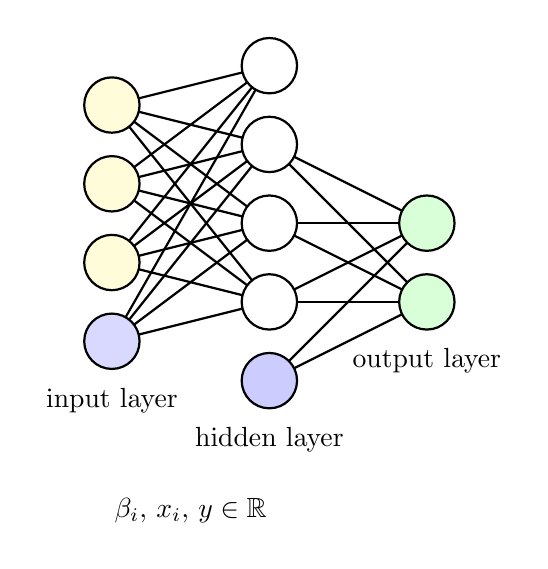
\begin{tikzpicture}
  \matrix[row sep=1em]
  {
      \foreach \i in {0, 1, 2, 3} {
        \foreach \j in {1, 2, 3, 4} {
          \draw[thick] (0, \i + 1.5) -- (2, {\j + 1});
        }
      }

      \foreach \i in {0, 1, 2, 3} {
        \foreach \j in {0, 1} {
          \draw[thick] (2, {\i + 1}) -- (4, \j + 2);
        }
      }

      \draw[thick, fill=blue!15] (0, 1.5) node {$$} circle (1em);
      \foreach \i in {1, 2, 3} {
        \draw[thick, fill=yellow!15] (0, \i + 1.5) node {$$} circle (1em);
      }
    
      \foreach \i in {0, 1} {
        \draw[thick, fill=green!15] (4, \i + 2) node {$$} circle (1em);
      }

      \draw[thick, fill=blue!20] (2, 1) node {$$} circle (1em);
      \foreach \i in {1, 2, 3, 4} {
        \draw[thick, fill=white] (2, \i + 1) node {$$} circle (1em);
      }

      \node at (0, 0.75) {input layer};
      \node at (2, 0.25) {hidden layer};
      \node at (4, 1.25) {output layer};
  \\
      \node at (1, 0) {$\beta_i,\, x_i,\, y\in\RR$}; \\
  };
  
\end{tikzpicture}
\end{document}